\section{Methodology}

This work utilized seven seminars presented during this semester, selected based on their order of presentation. The chosen seminars are as follows: 
\begin{itemize}
    \item "The Dawn of an Immersive Internet: XR, Generative AI and the Road to 6G" by Mischa Dohler
    \item "AGI Chips - The Next Frontier" by Alex James
    \item "Generalist vs Specialist Language Models" by Rodrigo Nogueira
    \item "From Intelligent Surfaces to Noise-Driven Communication: Innovative Technologies for 6G and Beyond" by Ertuğrul Başar
    \item "An Overview of Evolutionary Multi-Objective Optimization" by Carlos Artemio Coello Coello
    \item "Packet Trimming at the Edge for Low Latency in 6G Environments" by Stuart Clayman
    \item "Scientific Machine Learning and Quantum Utility: A Near Future Perspective" by Alberto Nogueira
\end{itemize}

The methodology followed several steps to collect, organize, and analyze data from these seminars. 

\subsection{Transcription of Seminar Videos}
The transcription of each seminar's YouTube video was obtained using the following steps:
\begin{itemize}
    \item First, the seminar video was opened on YouTube:
    \begin{figure}[H]
        \centering
        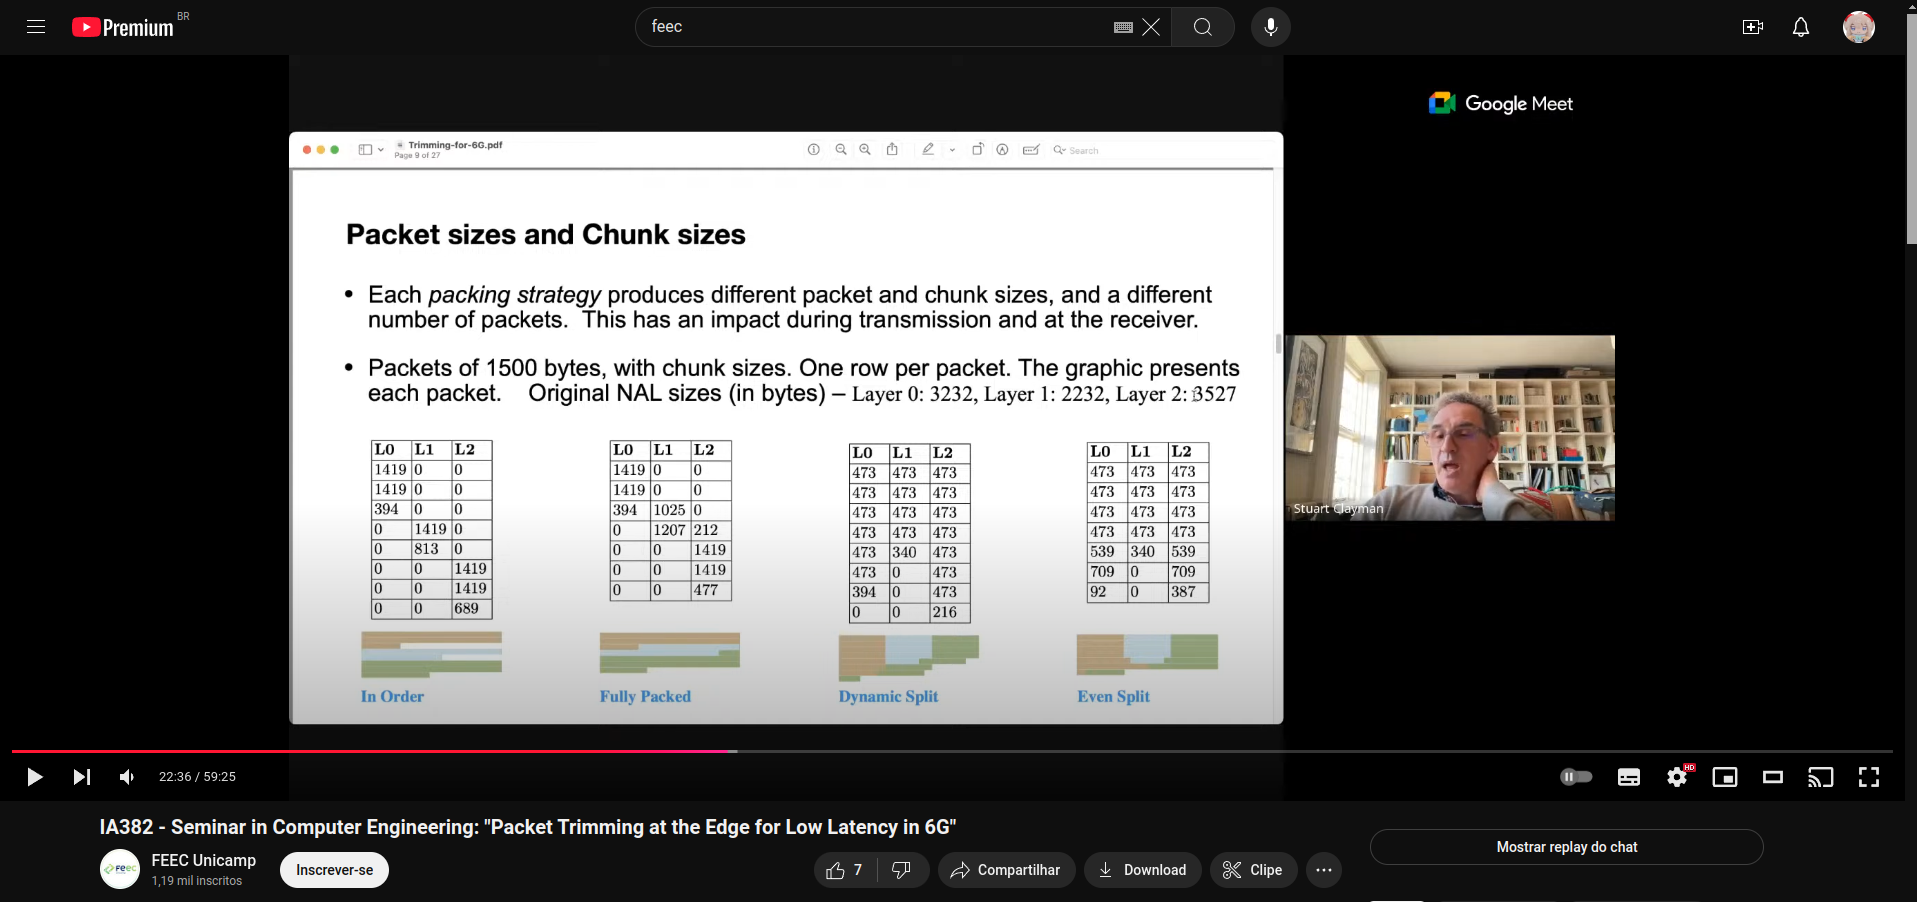
\includegraphics[scale=0.35]{Imagens/Youtube Example.png}
        \caption{Example of a seminar video on YouTube.}
    \end{figure}
    \item Then, the button to display the transcription was located in the video description. In the example below, YouTube was set to Portuguese, so the button displayed was "Mostrar Transcrição":
    \begin{figure}[H]
        \centering
        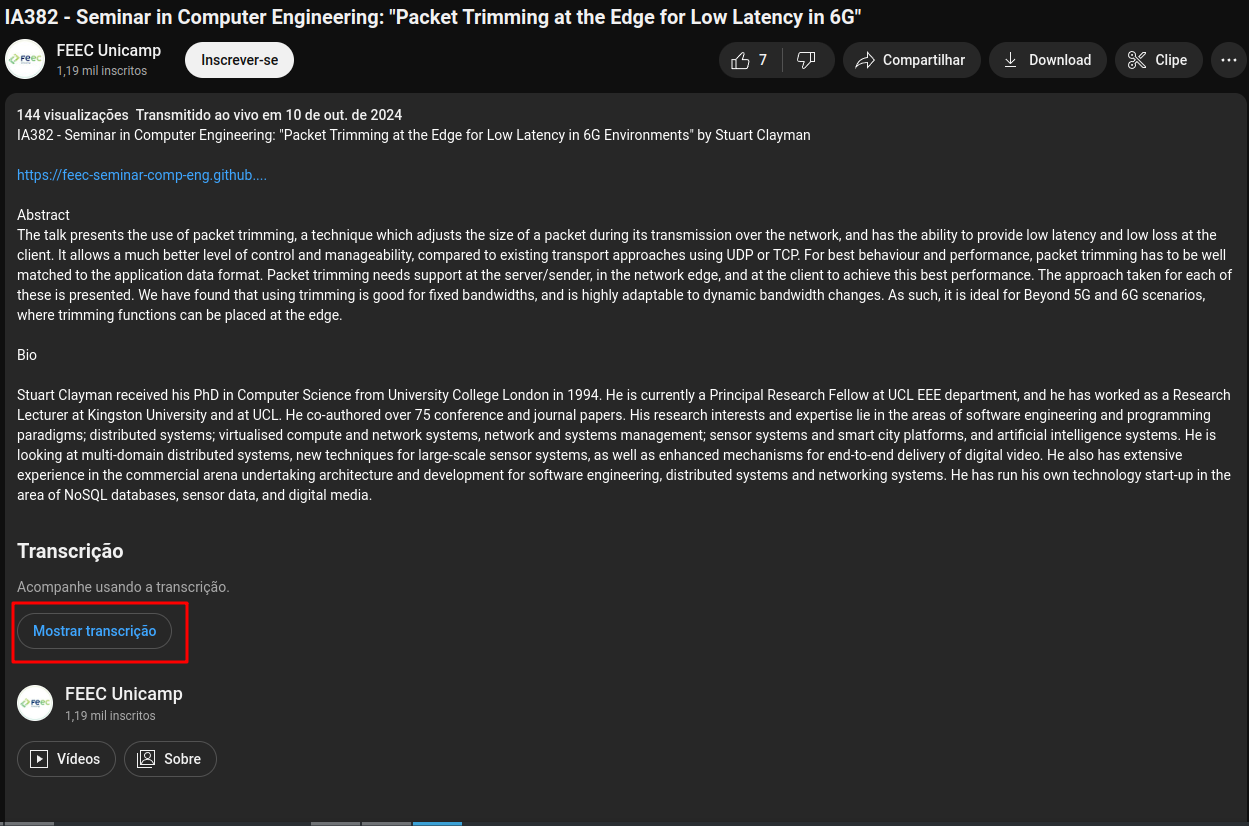
\includegraphics[scale=0.35]{Imagens/show trans.png}
        \caption{Button to show transcription in YouTube's interface.}
    \end{figure}
    \item Finally, the transcription was displayed and adjusted to show only the text:
    \begin{figure}[H]
        \centering
        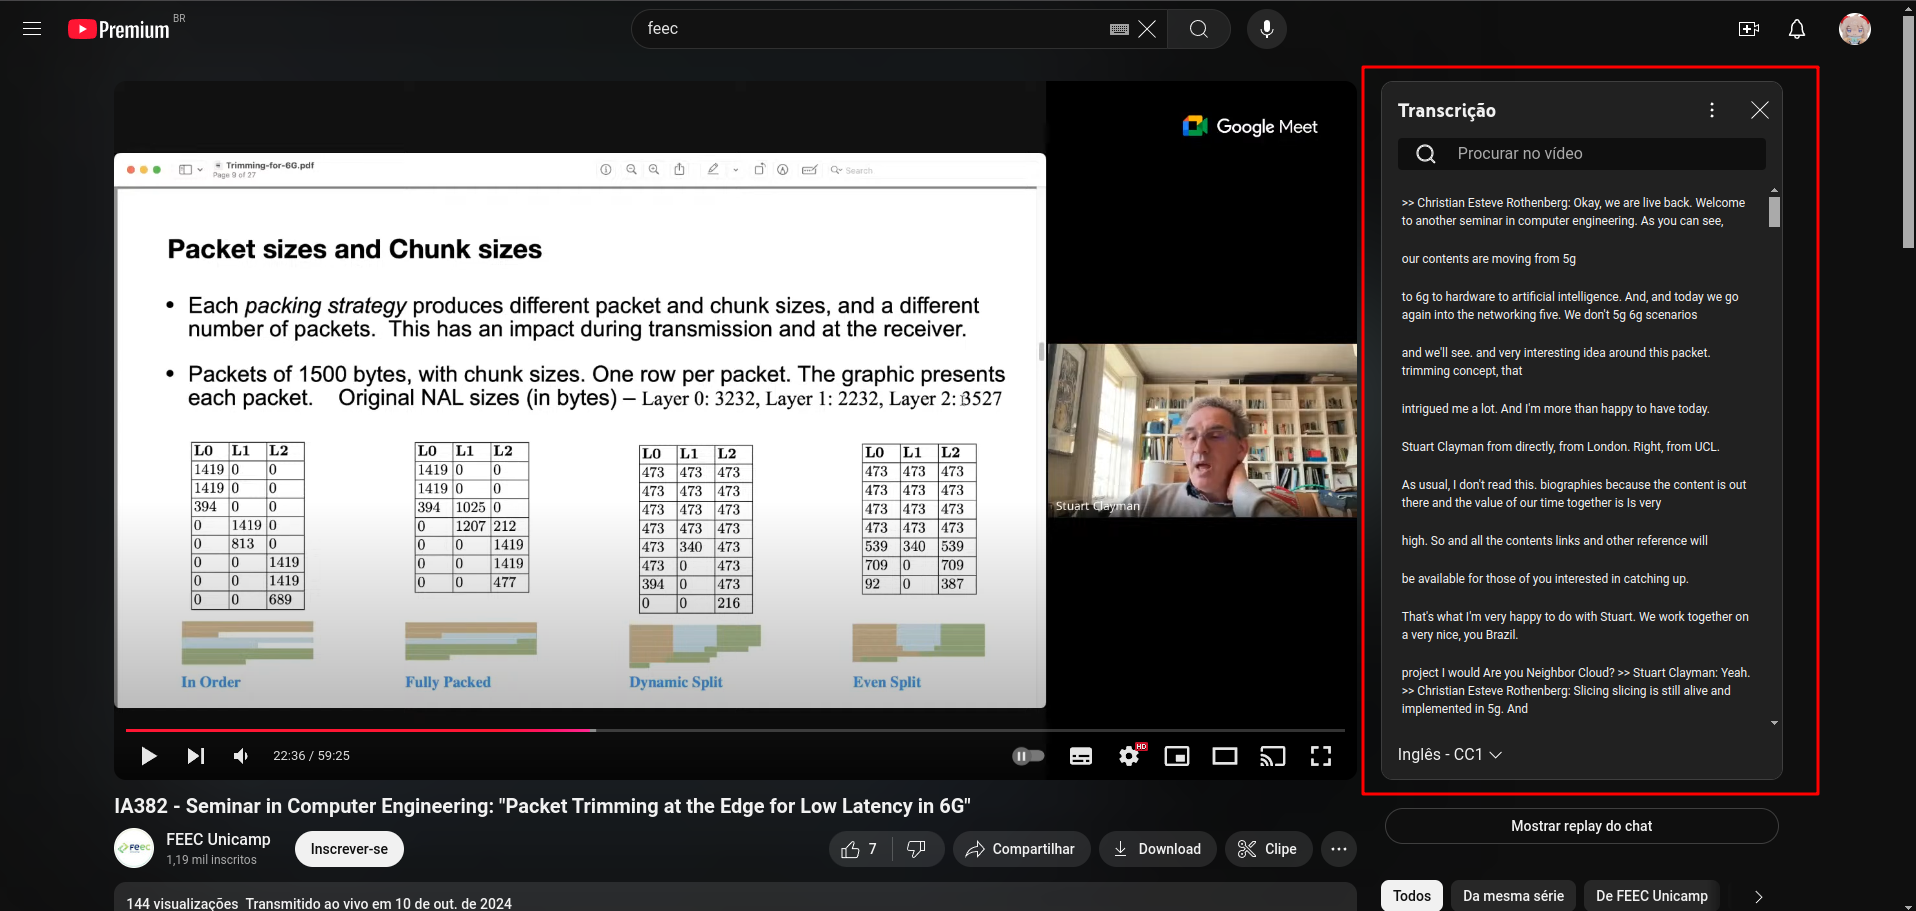
\includegraphics[scale=0.35]{Imagens/the trans.png}
        \caption{Extracted transcription of the seminar.}
    \end{figure}
\end{itemize}

\subsection{Creation of a Notebook for Data Organization}
The transcriptions were organized into a notebook using NotebookLM. Although 10 seminars were initially added, only the first seven were utilized in this study. 
\begin{figure}[H]
    \centering
    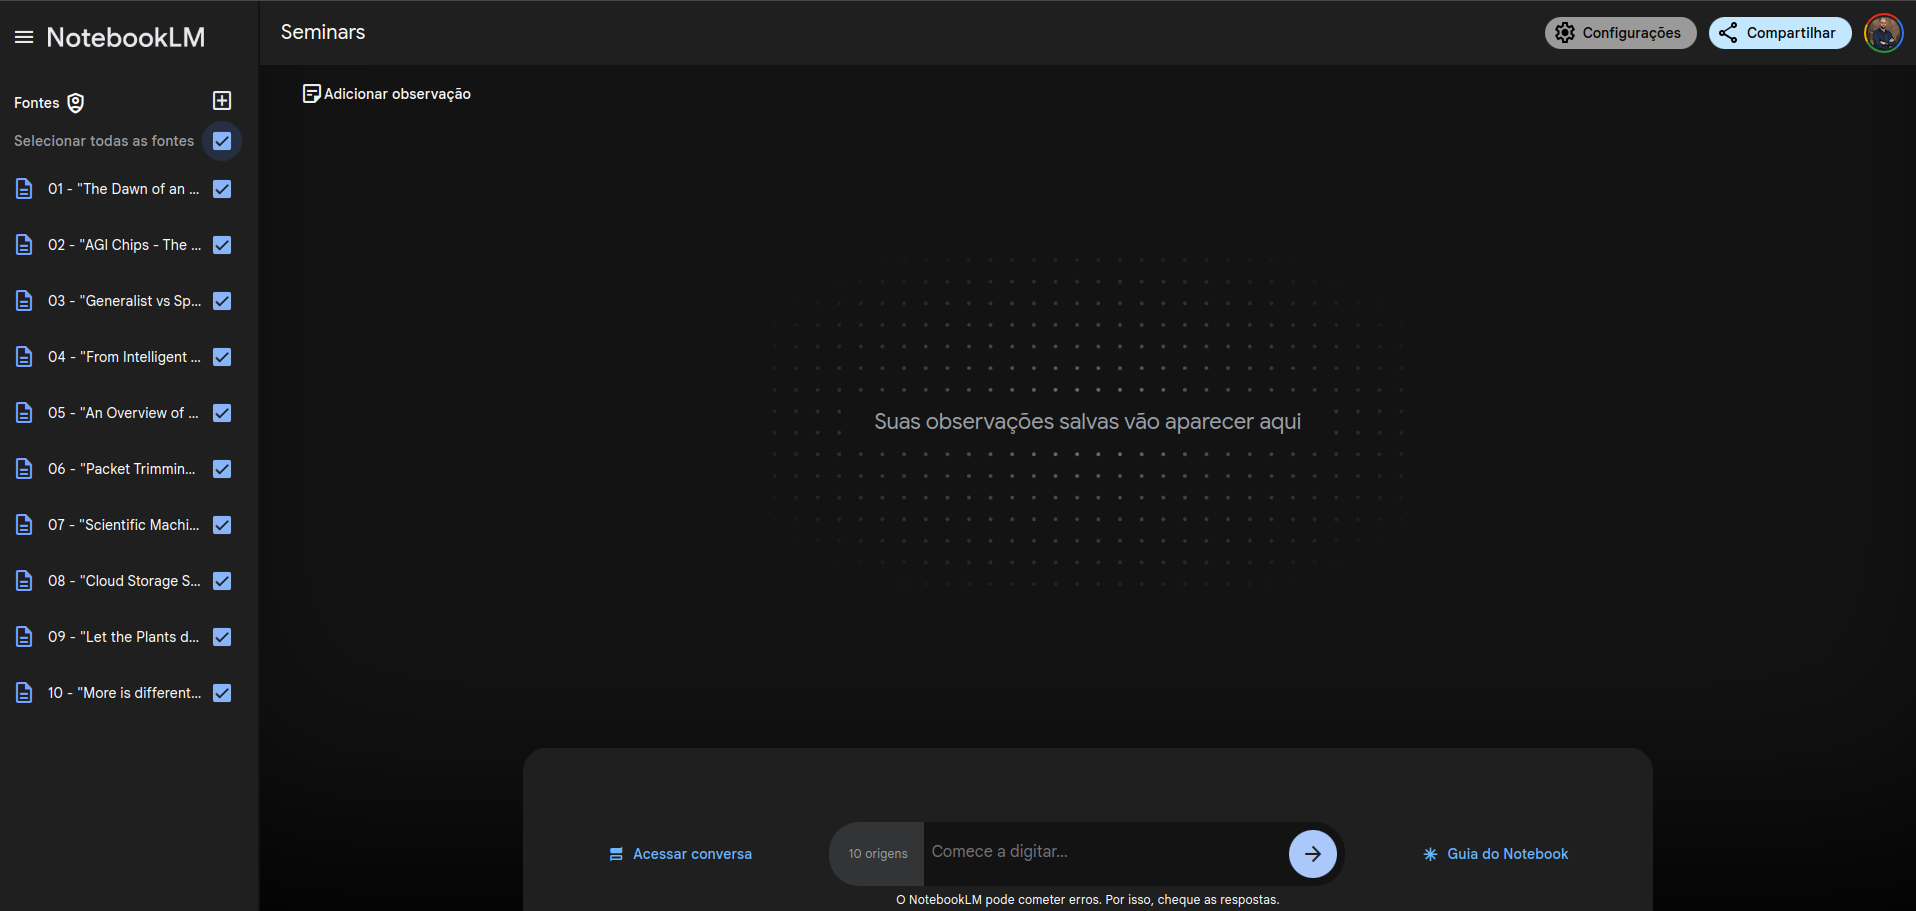
\includegraphics[scale=0.35]{Imagens/completed Notebook.png}
    \caption{Notebook created in NotebookLM containing seminar transcriptions.}
\end{figure}

\subsection{Generating Questions from Transcriptions}
Each seminar transcription was analyzed individually, and the following prompt was used: *"Give five questions about the seminar."* This restriction to five questions was made to streamline the analysis while providing sufficient data. An example of the process is shown below:
\begin{figure}[H]
    \centering
    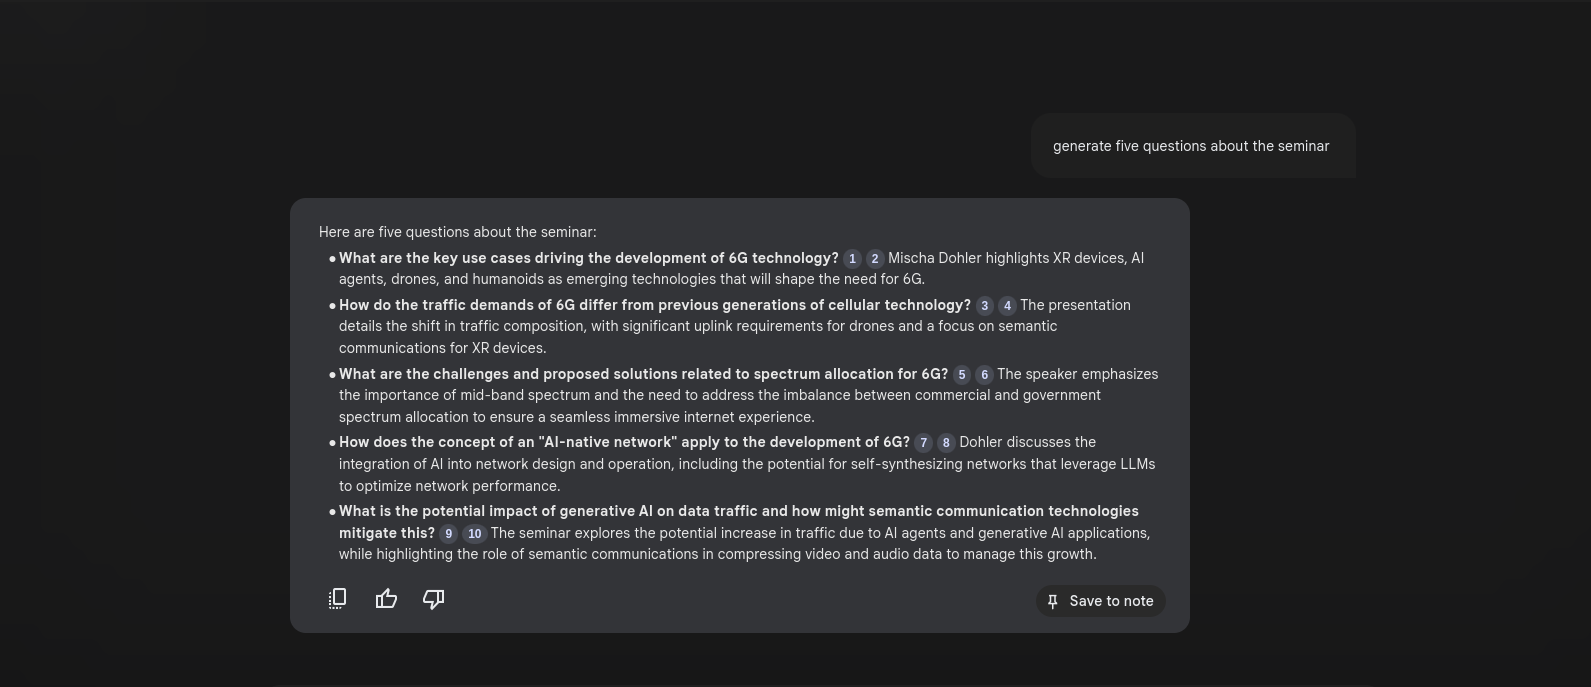
\includegraphics[scale=0.35]{Imagens/question.png}
    \caption{Example of a generated set of questions.}
\end{figure}
The generated questions were then formatted, removing any associated answers, as illustrated below:
\begin{tcolorbox}
What are the key use cases driving the development of 6G technology?\\
How do the traffic demands of 6G differ from previous generations of cellular technology?\\
What are the challenges and proposed solutions related to spectrum allocation for 6G?\\
How does the concept of an "AI-native network" apply to the development of 6G?\\
What is the potential impact of generative AI on data traffic, and how might semantic communication technologies mitigate this?\\
\end{tcolorbox}

\subsection{Obtaining AI Responses}
These questions were then submitted to ChatGPT, Gemini, and Meta AI, using the following prompt: 
\begin{quote}
"I want you to answer the following questions in English. I want short and direct answers."
\end{quote}
This phrasing ensured concise responses and standardized the language for analysis. An example interaction with ChatGPT is shown below:
\begin{figure}[H]
    \centering
    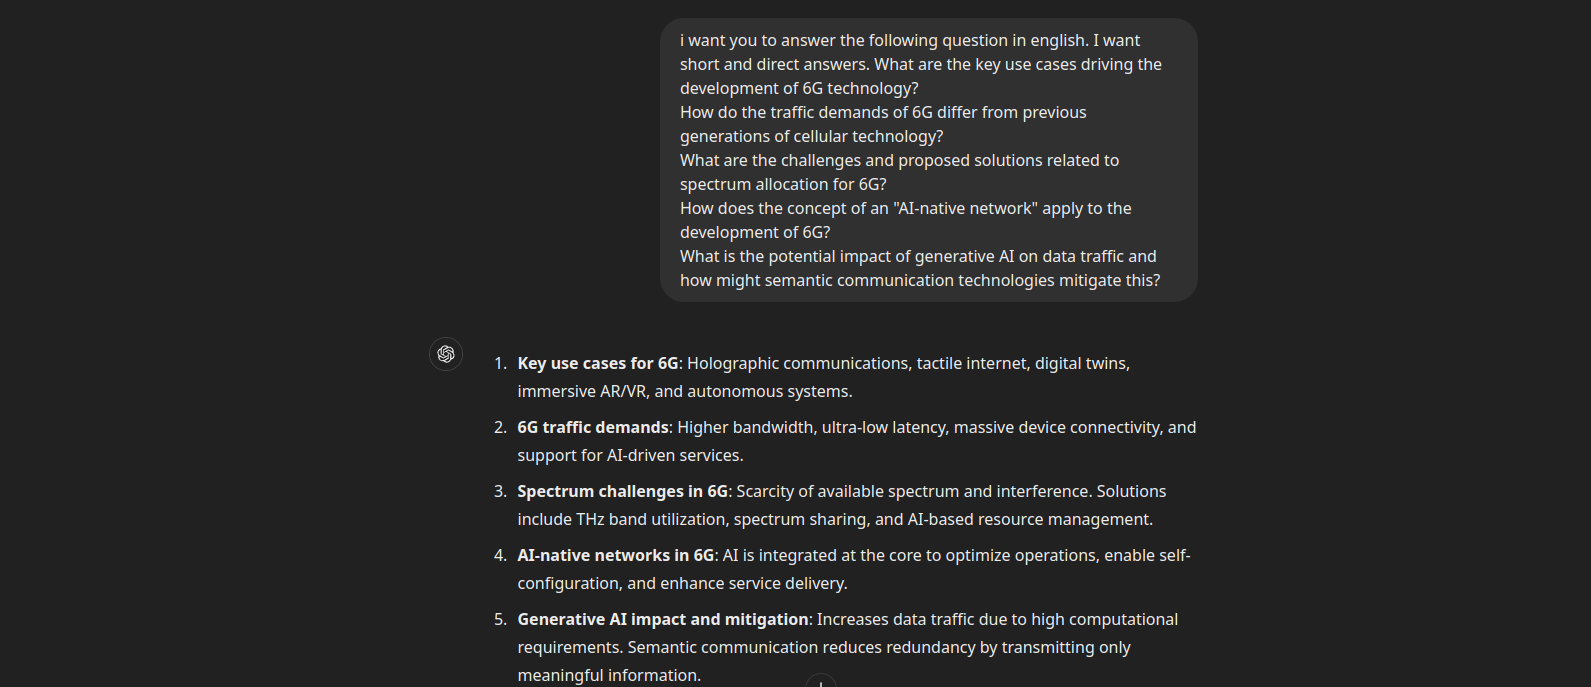
\includegraphics[scale=0.35]{Imagens/chatgpt.png}
    \caption{Example of AI-generated answers in ChatGPT.}
\end{figure}

\subsection{Correction and Scoring of Answers}
The AI-generated answers were then submitted to NotebookLM for correction. The following prompt preceded the submission:
\begin{quote}
"Correct these answers."
\end{quote}
An example is shown below:
\begin{figure}[H]
    \centering
    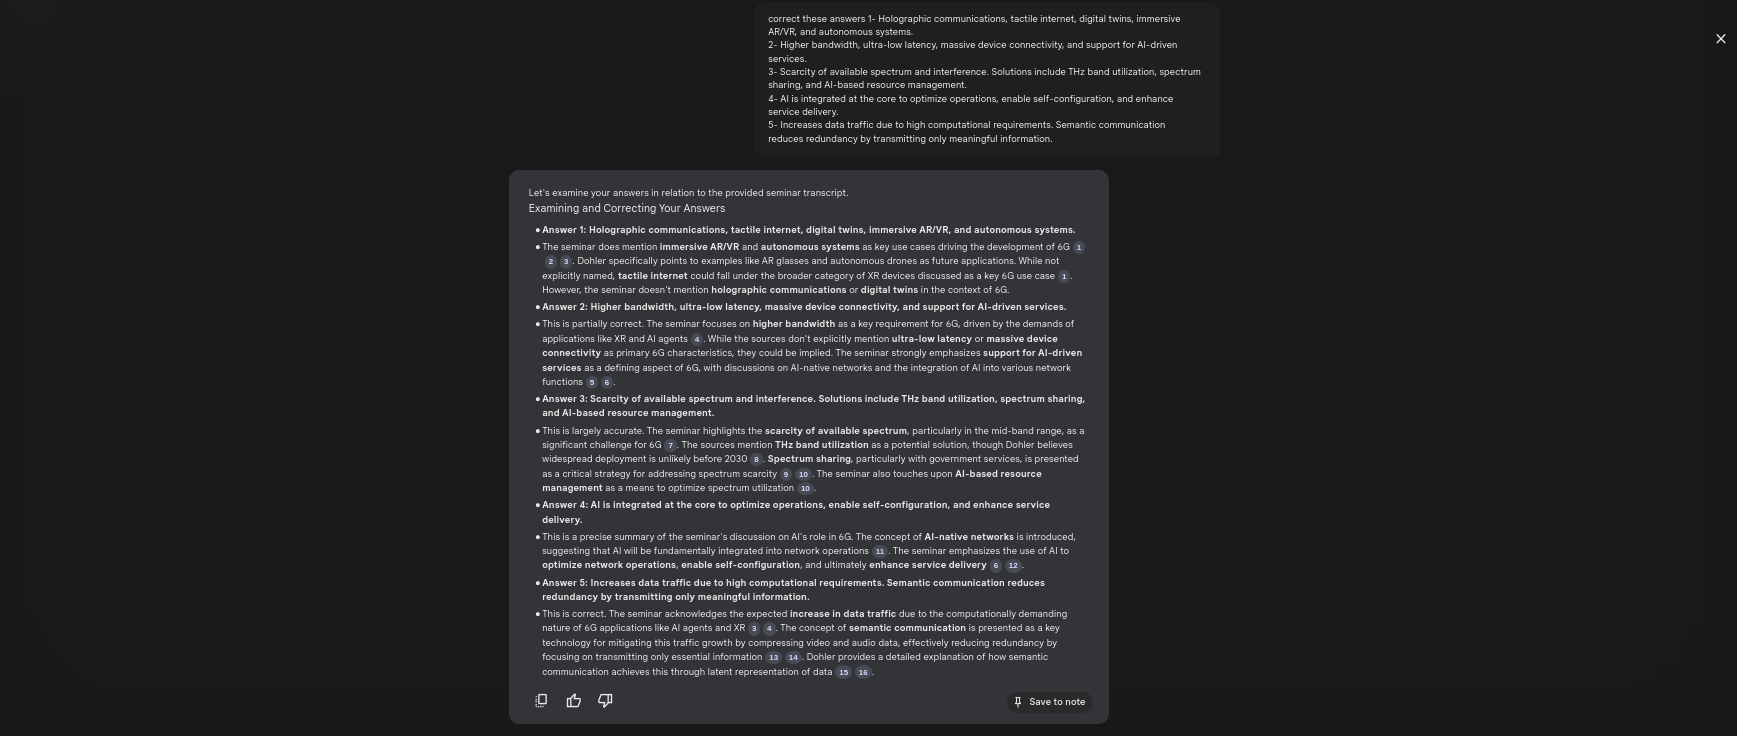
\includegraphics[scale=0.35]{Imagens/correction.png}
    \caption{Correction of AI-generated answers in NotebookLM.}
\end{figure}

The corrected responses were scored using a simple rubric:
\begin{itemize}
    \item Correct answers: +1 point
    \item Partially correct answers: +0.5 points
    \item Incorrect answers: 0 points
\end{itemize}

\subsection{Data Compilation and Visualization}
The results were compiled into a CSV file for analysis. This data was used to generate graphs to visualize performance trends across different AIs.
\subsection{Flowchart}
The following flowchart summaries the methodology:
\begin{figure}[H]
    \centering
    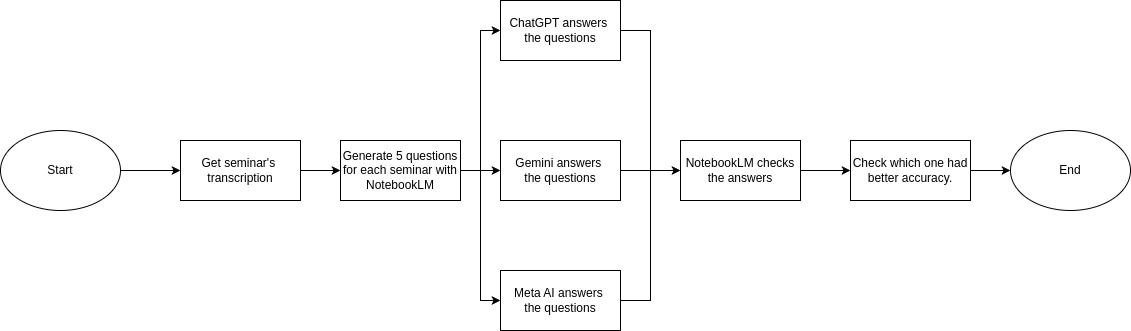
\includegraphics[scale=0.4]{Imagens/flowchart.jpg}
    \caption{Flowchart}
\end{figure}
\pagebreak